\documentclass{jot}

\usepackage[utf8]{inputenc}
%\usepackage[T1]{fontenc}
\usepackage[english]{babel}
\usepackage{microtype} % optional, for aesthetics
\usepackage{tabularx} % nice to have
\usepackage{booktabs} % necessary for style
\usepackage{graphicx}
% \graphicspath{{./figures/}}
\usepackage{listings}
% \lstset{...}

% \newcommand\code[1]{\texttt{#1}}
% \let\file\code

%%% Article metadata
\title{Reflections on OCL~2}
\runningtitle{Reflections on OCL~2}

\author[affiliation=orgname, nowrap] % , photo=FILE]
{Edward D. Willink}
{
	
Since parts of this paper rely on the personal observations of one of the leading participants at OMG and Eclipse, it is appropriate to provide a selective biography to distinguish my direct and indirect knowledge.
	
My involvement started in around 2003 from providing Eclipse support for the UMLX model transformation language~\cite{Willink-UMLX} using the then planned QVTr language. This led to participation in the Eclipse support for QVTr and interaction with the Eclipse OCL project~\cite{Eclipse-OCL} to make it extensible for use by the Eclipse QVTd project~\cite{Eclipse-QVTd}. I had no involvement with OCL~2.0. I contributed a few review comments to QVT~1.0.
	
Involvement with OCL and QVT at Eclipse led to the my appointment as the Thales representative for the OMG Revision Task Forces for OCL and QVT. I therefore contributed some revisions for OCL~2.2 and consistent models for QVT~1.1.
	
As personnel at OMG and Eclipse moved on, I found himself as chair of the OMG OCL and QVT RTFs and as project lead of Eclipse OCL and QVTd projects. Lack of active personnel meant that I was often the sole active participant.
	
I `retired' from Thales in 2012. Since then I am grateful, firstly to Tricia Balfe at Nomos Software, and then to Cory Casanave at Model Driven Solutions, for appointing me as their OCL and QVT RTF representatives.
	
At OMG, I resolved the `easy' problems in OCL~2.3 and OCL~2.4. This led to increasing awareness of the `hard' problems and the issuing of a Request For Proposal to address these via an `OCL~2.5' rewrite. The RFP~\cite{OCL-2.5-RFP}, starting at Section~6.5, can be read as a catalog of the serious OCL~2 problems.
	
At Eclipse, I inherited the Classic Eclipse OCL for Ecore/UML whose stable APIs made significant development almost impossible. A new fully-modeled Eclipse OCL exploited Xtext to provide much enhanced UX and a Pivot model to unify the competing Ecore and UML needs. Enhanced APIs, and Java code generation, support extension for QVT. The Pivot-based Eclipse OCL prototyped many solutions for OCL specification problems. Many of the solutions have been presented to the annual OCL Workshop. Unfortunately the need for API stability has become a hindrance to further development.
	
Contact him at \email{ed \_at\_ willink.me.uk}.}

\affiliation{orgname}{Willink Transformations Ltd., Reading, UK,}

\runningauthor{Edward D. Willink}

\jotdetails{
	volume=V,
	number=N,
	articleno=M,
	year=2011,
	doisuffix=jot.201Y.VV.N.aN,
	license=ccbynd % choose from ccby, ccbynd, ccbyncnd
}

\begin{document}

\begin{abstract}
	
Twenty years after the OCL~2.0 Request For Proposals, it is perhaps long overdue for a review as to how well the resulting semi-formal OCL~2 specification makes the informal OCL~1 specification more precise. We briefly relate the history that allowed an imprecise draft to be adopted by the OMG as the OCL~2.0 specification resulting in a language that was fatally flawed from the outset. We draw on personal experience to explain why recognition of the fatality of the flaws has taken so long. However despite these flaws, OCL remains the language of choice for specifying model constraints. Therefore armed with an understanding of the flaws, we make practical suggestions for how an OCL~3.0 might resolve them.

\end{abstract}

\keywords{OCL, Object Constraint Language, Precise specification, Side effect free}

\section{Introduction}

The UML specification arose to resolve the `method wars' that left users confused as to whether a class should be drawn as a cloud or rectangle. In this respect UML has been a total success, but obviously there is more to modeling than classes, and as soon as models become non-trivial, additional constraints are required that cannot be sensibly expressed graphically. The UML~1.1~\cite{UML-1.1} suite of documents therefore includes a document defining the OCL~1.1~\cite{OCL-1.1} textual language that can elaborate UML diagrams.

The OCL language evolved from work on the Syntropy method at IBM, and in so far as many thousands of academic papers have successfully used OCL to express constraints, OCL too has been a total success.

Unfortunately the prevailing state of the OCL specification is very unsatisfactory leading to incompatibility between implementations and difficulty in creating new ones. We will argue that we need to make the credible not only to support the full potential of OCL but also to support lightweight research activities. 

In Section~\ref{History} we relate the history of the OCL~1 to OCL~2 transition before examining the problems with OCL~2. Then in Section~\ref{Problems} we examine these problems that variously emanate from the language, usability, the specification or typical tooling and identify solutions to the problems. Some evolution beyond the specification is described in Section~\ref{Evolution} culminating in some suggestions in Section~\ref{OCL~3 tooling Proposal} as to how to specify a much simpler OCL~3. Finally in Section~\ref{Conclusion} we conclude.

\section{OCL~1 to OCL~2 History}\label{History}

The software community was not satisfied to leave UML~1 (and OCL~1) as a useful flexible semi-formal facility for communicating analysis considerations. Rather a near-formal semantics for UML~2 (and OCL~2) was required to specify behavior precisely and so facilitate synthesis of functional code direct from UML diagrams. 

The formality of OCL was addressed by Martin Gogolla's student Mark Richters whose PhD thesis~\cite{Richters} was adapted to provide the formal Annex that accompanies all the OCL~2.x specifications. It provides a useful reference to help resolve issues in the main specification, however since the Annex has not tracked all the OCL~2 evolutions, sometimes the Annex just contributes to a contradiction for implementers and users to reconcile.

\subsection{OCL~1.5}

Reviewing the final version of the OCL~1 specification embedded within the UML~1.5 specification~\cite{UML-1.5}, we find a nice simple 50 page informal exposition of:
\begin{itemize}
	\item{the language from a user perspective}
	\item{the library operations from a user perspective}
	\item{an EBNF grammar}
\end{itemize}

This could be called a black box specification. It reveals what the user sees. It imposes no limitations on how an implementation satisfies the specification. With so little detail, most of the problems of the 210 page OCL~2.0~\cite{OCL-2.0} do not exist. However some do.

OCL~1 uses open classes in so far as let-operations and let-attributes define new pseudo-operations and pseudo-attributes for the exclusive use of the OCL. No clues are provided about how pseudo-operations and pseudo-attributes are modeled by UML's closed classes.

OCL~1.5 claims that `A parser generated from this grammar has correctly parsed all the constraints in the UML Semantics section, a process which improved the correctness of the specifications for OCL and UML.' This is patently untrue since, skipping over obvious formatting typos such as the \verb$Guard$ invariant, many of the constraints have failed to track the language evolution that mandates empty parentheses on parameterless operations and replaces the \verb$#$ syntax for enumerations by qualified names.

%UML~1.x has \verb$Attribute$s, \verb$AssociationEnd$s, \verb$Operation$s and \verb$Method$s for which OCL~1 uses the generic term `property'. Unfortunately when UML~2.0 unified the \verb$Attribute$ and \verb$AssociationEnd$ classes as the \verb$Property$ class, the OCL text failed to track uniformly; the resulting OCL~2 text can be rather confusing.

OCL~1 uses the term `stereotype' to refer to the \verb$inv$/\verb$pre$/\verb$post$ discriminant. This is confusing to any reader who may be familiar with the UML \verb$Stereotype$ class and its capabilities.

OCL~1 specifies that all collections are always flattened.

OCL~1 recognizes that non-collection values may be `null', but does not provide any clues as to what this may mean semantically.

OCL~1 does not specify what happens if the index-is-in-range precondition for \verb$Sequence::at$ is not satisfied. OCL~1 does not specify a no-divide-by-zero precondition on \verb$Real::/$.

OCL~1 specifies that the Standard Library is a modeled \verb$Package$ and specifies how it may be extended by another \verb$Package$ using an \verb$«OCL_Types»$ dependency. No model for the Standard Library is provided and so the specified extension is not practical. 

\subsection{UML~2.0 submissions}

The two competing UML~2.0 submissions~\cite{UML-2U},\cite{UML-U2P} both recognized the utility of OCL and also recognized that OCL had utility beyond UML. OCL was therefore excluded from the responses to the UML 2.0 RFP~\cite{UML-2.0-RFP} and treated as a new self-standing specification with its own RFP~\cite{OCL-2.0-RFP}. This separation was very convenient for the UML teams and in many respects good for OCL too, but unfortunately the separation from UML and the drive to better formality required many extra problems to be addressed. When the UML teams ran out of enthusiasm / resources, the result was a work in progress draft~\cite{OCL-2.0-draft}.

The draft OCL sat on the shelf at OMG for three years until seven out of eight of the competing QVT specification submissions agreed that the QVT specification should exploit OCL. The QVT specification~\cite{QVT-1.0} could not be adopted until the OCL~2.0 specification had been adopted and so the work in progress draft was dusted off, polished slightly and adopted leading to the official OCL~2.0~\cite{OCL-2.0}. It is unclear how this could have happened since the draft clearly lacked the prototyping required by OMG, and contains many TBDs (To Be Decided) once UML~2.0 was finalized. UML~2.0~\cite{UML-2.0-adopted} was of course adopted three years prior to this OCL~2.0 adoption. The TBDs persist to this day and are even present in OCL~2.3.1~\cite{OCL-2.3.1} which was adopted as an ISO standard; perhaps the only ISO standard with explicit TBDs and prolific known inconsistencies.

\subsection{OCL~2.0 aspirations}\label{OCL~2.0 aspirations}

Whereas OCL~1.x was a black box specification, OCL~2.x is a white box specification. It specifies the Abstract Syntax (AS) model for OCL with the excellent intention that this should facilitate interchange using XMI between alternative OCL tools. Unfortunately this model was not provided until OCL~2.2~\cite{OCL-2.2} and even then it is not quite right since no prototype had been built.

As an evolution of OCL~1.x, it was natural for the OCL AS model to re-use UML metaclasses. However once the UML-OCL connection was severed, the use of such a bloated and in some respects inadequate foundation should have been reconsidered. The re-use of UML became untenable once OCL~2.0 Section 13 added the claim that EssentialOCL could work with EMOF.

Specification of the AS model required that the conversion between the grammar and the AS be specified as well. This is achieved by specifying a non-normative Concrete Syntax (CS) model that closely resembles the grammar, and a variety of rules mapping the grammar to CS and the CS to AS. Since the grammar is ambiguous, a further category of disambiguating rules is required. The exposition of this conversion burden is arranged around the non-normative CS classes, for which no model has been provided. This avoids revealing how far from correct the CS classes are. The coherent OCL~1.5 grammar is replaced by CS-relevant snippets scattered throughout the chapter. As a minimum this imposes a major cut and paste burden on any developer attempting to use them. More practically, it obfuscates to such an extent that a casual reader is impressed by the apparent detailed formality and unaware of the total absence of any prototyping to substantiate the unusable content.

Standardization of the AS requires that the internal awkwardness of OCL~1.x's pseudo-attributes and pseudo-operations be properly modeled. They are not and to make matters worse the pseudo-attributes and pseudo-operations are elevated to attributes and operations that can be used just as if they were part of the original model. This is tantamount to providing open classes and presents an unresolved challenge when the AS model based on UML's closed classes is serialized as XMI.

The availability of an AS model provided an opportunity to specify the execution semantics. The exposition is semi-formal and uses a rather obvious and incomplete \verb$ValuesPackage$ and \verb$EvaluationPackage$. %How can if-then-else be specified without presupposing its semantics? \verb$IfExpEval$ avoids the problem by leaving the condition/then/else to result value relationships to the readers intuition.

The \verb$EvaluationPackage$ makes a first attempt at temporal modeling using a \verb$LocalSnapshot$ class to maintain a history of object states. I'm not aware of any implementation that uses this aspect of the specification. The relatively recent work on sequences of system snapshots (filmstrips~\cite{Desai}) by Martin Gogolla's team at Bremen~\cite{USE} seems much more promising.

\subsection{OCL~2 Architecture}

\begin{figure}
	\begin{center}
		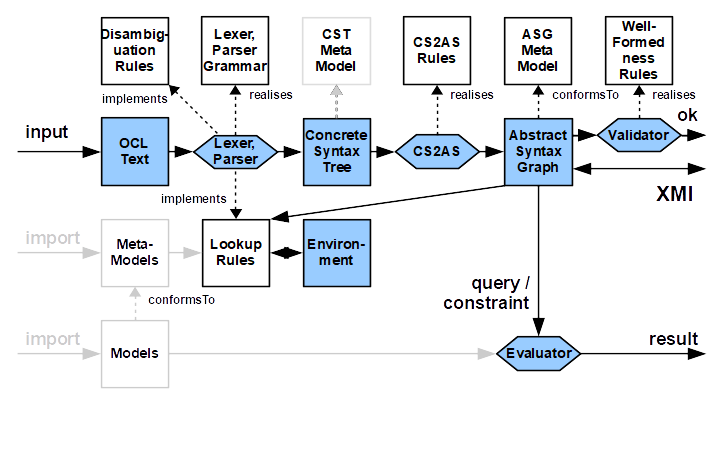
\includegraphics[width=4.5in]{OCL2Architecture.png}
	\end{center}
    \vspace{-40pt}
	\caption{OCL~2 Architecture}
	\label{fig:OCL2Architecture}
\end{figure}

Fig~\ref{fig:OCL2Architecture} shows the components of the architecture implied by the specification. Along the top row, transparent boxes show different aspects of specified behavior that configure the shaded concrete boxes realized by the tooling on the second row. Input text is lexed and parsed to give a Concrete Syntax Tree that is converted to an Abstract Syntax Graph and then validated.

The troublesome ability to interchange the ASG using XMI is indicated.

A non-standard parser is required since it must implement the disambiguation rules and lookup rules. The lookup rules cannot be expressed in pure OCL since they create and modify new \verb$Environment$s for each construct such as a \verb$LetExp$ that introduces a nested scope. The mechanism by which the user-metamodels are imported and the construction of a root \verb$Environment$ is greyed out since it is unspecified.

The bottom row shows how the parsed ASG provides a query or constraint that an evaluator may use to provide a result, using models whose import mechanism is again unspecified.

Before criticizing OCL~2 too harshly, it must be remembered that there were no metamodels for OCL~1 and so the metamodels for OCL~2 were a significant novelty. We could praise the OCL~2 metamodels for being perhaps 95\% correct rather than dwelling on the 5\% wrong. However it is the 5\% wrong and the lack of a comprehensive prototype to reveal the wrongness that has caused so much trouble for implementers whose trust in the OMG specification was misplaced.

\section{Problems}\label{Problems}

The problems with OCL take many forms. In the following subsections we categorize them to distinguish those that directly affect users and those which only affect toolsmiths struggling to make sense of the specification.  

\subsection{Language Problems}

Problems with the OCL language have a very direct impact on the user and may require users to program in an unnatural style to circumvent the limitations.  

\subsubsection{Program Failure}

An inevitable characteristic of any manually developed program is that it may malfunction and consequently the program language and execution support must accommodate failures. Failures typically take one of three forms.

\paragraph{Catastrophic failure} A catastrophic failure is often called a crash. It may occur from a hardware, software, network, or I/O system failure. Programs cannot normally recover from crashes and so the execution launcher will attempt to provide as much helpful diagnosis of the crash as possible before terminating execution abruptly.

\paragraph{Recoverable failure} A recoverable failure may occur when the programmer finds it convenient to reuse some failure detection code and then to compensate for the failure, typically by catching a thrown exception.

%exploit failure detection within some invoked module than to duplicate the detections and so avoid the failure. A simple example of this occurs when a Java \verb$NumberFormatException$ is caught after using \verb$Double.parseDouble$ to convert a string representation of a number to a number. In this case programming a syntax check would be a waste of effort and execution time.

\paragraph{Not-a-failure} Conversely a programmer may correctly anticipate a failure and provide a guard to direct the program control to bypass and so avoid the failure. 

In Java the two actual failure cases are separated by using a \verb$RuntimeException$ or an \verb$Error$ for catastrophic failures and by using \verb$Exception$ for recoverable failures. \verb$Exception$s form part of a Java function signature and so there can be some static diagnosis of code that neglects to handle the recoverable failures.

OCL~1 has preconditions but provides no indication of how an evaluation should behave when a precondition is not satisfied. OCL~2 is similarly vague and so OCL~2 tools often treat the corresponding preconditions (and postconditions) as just syntax-checked comments to document a hazard for a human reader.

OCL~2 pursues a functional approach and, in the event of a malfunction, returns a regular \verb$invalid$ value rather than imposing an alternative `return' mechanism for an \verb$Exception$. The \verb$invalid$ value can be `caught' by using the \verb$oclIsInvalid()$ library function. This is different to many languages but is more regular and so perhaps better.

Unfortunately the OCL~2 specification is not really concerned with failures for which it mandates that \verb$invalid$ is a singleton; all failures are the same and free from any helpful diagnostic detail. Some OCL tools ignore this pointless restriction and provide a rich \verb$invalid$ that propagates diagnostics while preserving OCL semantics by ensuring that the diverse \verb$invalid$s behave as one.

The lack of consideration for crashes forces an OCL~2 implementer to use the \verb$invalid$ return for crashes.% and to ensure that they can be caught be \verb$oclInInvalid()$.

The OCL specification provides no ability for the use of \verb$invalid$ to be declared as part of a function signature, consequently OCL, whose strong side effect free formality supports strong analysis, has a gaping hole in regard to guaranteeing that a program execution will not fail.

\paragraph{Resolution} Elevating a crash to a strict behavior is a straightforward change hampered only by a perceived resistance to expanding Booleans to 5-values: \{\verb$true$, \verb$false$, \verb$null$, \verb$invalid$, \verb$crash$\}. It should be recognized that these five values only occur for malfunctioning programs. See Section~\ref{Fail-Safe OCL} for work on proving that these malfunctions cannot occur and so proving that the programmed Boolean computation is indeed internally 2-valued. 

\subsubsection{Import, Extensibility, Modularization}

OCL is an unusual language in that by itself it is almost completely useless. It only becomes useful once embedded in an environment that provides models upon which OCL computations can operate.

The only partially specified practical usage of OCL is the Complete OCL extension that enables an OCL document to complement some pre-existing metamodel with

\begin{itemize}
	\item constraints for UML classes
	\item pre/post-conditions/bodies for UML Operations
	\item initializers for UML Properties
	\item guards for UML Transitions
\end{itemize}

Clearly the Complete OCL document must be tightly coupled to some UML model, but unfortunately there is no `import' declaration. This forces all tools to invent a proprietary solution. 

Beyond the OCL specification, OCL is used as the basis for many model transformation languages such as QVT that provide the requisite models for the OCL queries and provide a disciplined mechanism by which the results of side effect free OCL queries provoke mutation of the models.

Unfortunately, the historic support for UML leaves OCL bloated with Message functionality that few tools support and State functionality that few users need. For pure OCL usage, this bloat can just be ignored, but for extended applications such as QVT this bloat is an embarrassment that should be removable. Conversely there are research areas such as Temporal specification for which researchers should be able to experiment with alternative temporal expressions.

\paragraph{Resolution}

The Pivot-based Eclipse OCL prototype adds an `import' declaration for use by OCL or QVT or ... The statement can be used to declare not only the metamodel(s) which the OCL complements but an optionally extended Standard Library that supplies re-usable functionality.

The models provided by the overall OCL specification should be structured in cross-cutting modules so that a tool may select a subset of the standard modules and augment with its own modules, thereby excluding unwanted Message and Tuple support while adding experimental Time support.

\subsubsection{Flattened Collections}

OCL~1 collections provide support for UML's multi-valued properties and since UML has no support for nested multi-values, OCL~1 collections were specified to avoid nesting by flattening at every opportunity. This mistake was partially recognized when OCL~2 introduced the \verb$collectNested$ iteration and the \verb$flatten$ operation. However this leads to a confusion requiring special efforts to avoid type corruption.

\paragraph{Resolution} All OCL collection operations should be type consistent so that a type conversion only occurs when the \verb$flatten$ operation is used explicitly.

\subsubsection{Collection conforms to OclAny}

The formalization in the OCL~2 Annex clearly states that the formalization applies to a type system in which Collections and Objects are distinct. It does not prohibit a unification, but observes that extra formalization effort is needed by a unification.

The OCL~2.2 specification changed to allow a \verb$Collection$ to conform to \verb$OclAny$ without putting in that extra effort or indeed even providing a use case to motivate the change.

Two possible use cases involve either defining a utility operation such as \verb$printf$ that can receive a polymorphic mix of collections and objects or to provide a stronger type than \verb$Collection(OclAny)$ for a heterogeneous nested collection. The latter challenge is perhaps where work in needed in the Annex.

\paragraph{Resolution} The conformance of \verb$Collection$ to \verb$OclAny$ does not seem to offer significant benefits, so it may be best to revert this change until the formalization work is done to understand its consequences. 

\subsection{Perceived Problem}

Not all problems are really problems at all.

\subsubsection{2-valued Booleans and invalid}

Almost every gathering of the OCL community provokes discussion of why OCL Booleans are not 2-valued \{\verb$true$, \verb$false$\}. Clearly many OCL users are unhappy with the prevailing 3-valued \{\verb$true$, \verb$false$, \verb$invalid$\} specification\footnote{The idempotent addition of null as a fourth output in OCL~2.4 is not relevant here.}.

But this is all a misunderstanding. In OCL, as in other languages, a non-trivial Boolean-valued calculation has three possible outcomes; success/\verb$true$, failure/\verb$false$ and crash/\verb$invalid$. When the crash is realized as a thrown exception, the programmer can ignore the crash outcome and code as if there were only two possible outcomes. Exactly the same programming approach is possible with OCL provided the programmer ensures that the particular OCL tooling API
%such as \verb$check()$
that is used for the evaluation is `strict'; i.e. it converts the \verb$invalid$ or \verb$null$ value returned by OCL to a crash by throwing an exception. The OCL tooling may offer an alternative API %such as \verb$evaluate()$
that returns all three outcomes as OCL values. This alternative is useful when the programmer really wants to exploit all three outcomes. An inappropriate choice of API is the probable source of unhappiness when only two outcomes are expected.

\subsection{Usability Problems}

Some aspects of the OCL language, even when adequately specified, have been found to cause undue difficulties for OCL users.

\subsubsection{Dot and Arrow Navigation operators}

Newcomers to OCL are confused by the difference between dot and arrow navigation operators. Prior to OCL~2.4, the specification was unhelpful and so newcomers fail to discover the simple rule that dot is for objects and arrow for collections. The availability of the implicit-collect and implicit-as-set short-forms give the dot and arrow operators a utility for the `wrong' sources. This can confuse even experienced OCL programmers.

\begin{verbatim}
    myCollection->collect(name)      -- explicit collect
    myAggregate.name                 -- ?? implicit collect ??
\end{verbatim}

The utility of implicit-collect is mixed. Some users like the compact exposition of some constraints. Other users dislike the ease with which a typo acquires an unexpected meaning. In the second example above, the use of a singular word such as \verb$myAggregate$ makes it impossible to tell locally whether \verb$name$ is a property access of the \verb$myAggregate$ instance of a \verb$MyAggregate$ class, or an implicit collect of the elements of a \verb$myAggregate$ collection.

Prior to OCL~2.4, the implicit-as-set was ill-specified and not a short-form The introduction of the explicit \verb$oclAsSet$ library operation formalized the short-form

\paragraph{Resolution}

The EOL variant of OCL used by the Epsilon~\cite{Eclipse-Epsilon} transformation languages demonstrates that it is possible to make do with just a dot operator for both object and collection navigations. The user confusions are eliminated.

A clearer OCL could similarly use just a dot operator. The brevity of implicit-collect could be rescued by defining a \verb$*.$ navigation operator which reads naturally as many-dot for an implicit-collect short-form

\begin{verbatim}
    myAggregate*.name                 -- short-form explicit collect
\end{verbatim}

A similar \verb$.*$ short-form which reads as dot-to-many could rescue the implicit-as-set, but this usage is probably too rare to merit the short-form

%\subsection{Precision}
%UML misdirection
%Model
%-- URI

%\subsection{Library}\label{Library}
%Utility
%Types
%Extensibility

\subsubsection{Implicit Source}

\paragraph{implicit-self} OCL, like many Object Oriented languages, allows the \verb$self$ start point of a navigation to be omitted. Since the \verb$self$ context is so important, this is very reasonable and can improve readability.

\begin{verbatim}
    name                 -- self.name
\end{verbatim}

\paragraph{implicit-source} OCL, unlike other languages, has powerful collection iteration capabilities and allows the start point of a navigation from an iterator to be omitted.

\begin{verbatim}
    aCollection->isUnique(name)   -- aCollection->isUnique(e | e.name)
\end{verbatim}

This again may aid readability by shortening the exposition. Unfortunately it also adds confusion since the tool and a reader must decide which of many possible implicit-sources in a nest of multi-iterator iterations or an implicit-self has been omitted. Typos and misunderstandings are too easy.

\paragraph{Resolution}

Within iterator bodies, only the first iterator of the most nested iteration should be available as an implicit source, self should be explicit.

\subsubsection{OCL Re-Use Cases}

The liberation of OCL from UML was intended to make OCL more generally useful. It is therefore particularly irritating when a user asks `how can I re-use OCL in my application?' This is irritating because the honest answer is that you can't unless you devote considerable skilled programming effort. Why is it so hard?

We first examine a couple of use cases that OCL could respond to and then look at how OCL could make them much easier.

\paragraph{Novel Application re-using OCL}

If the user has a novel application such as using OCL as a replacement for XPath in the XML/XSD technology space, there are two obvious choices.

\paragraph{Re-implement} A custom implementation can obviously satisfy all the user's requirements, but it requires the user to become familiar with all the complexities of OCL and to rediscover solutions to the many inadequacies of the OCL specification.

\paragraph{Re-Use} Re-use of existing functionality is often preferable, particularly if a re-usable implementation is available. Unfortunately the lack of a clear architecture in the specification encourages the proprietary struggles for solutions to pervade the implementation. It is not re-usable.

Wilke~\cite{Wilke-Variability} highlighted the lack of architecture nicely by identifying that an OCL implementer had two significant design choices to accommodate the user's preferred metamodel representation (UML, Ecore, XSD, Java, ...) and a further two design choices for the user's preferred model representation (Ecore, XML, Java, ...).

\paragraph{Denormalized metamodels} If the OCL functionality is to specify expressions for a particular metamodel representation, the OCL tooling can be coded specifically for that representation. In practice this means substantial re-tooling for each new metamodel representation. When the Classic Eclipse OCL support for Ecore was enhanced to support UML as well, an attempt was made to mitigate the costs of this re-tooling by introducing long (ten) template parameter lists and a reflective class to polymorphize the non-polymorphic Ecore/UML classes. This led to unpleasant code for all representations and probably made the prospect of supporting a third representation even more daunting.

\paragraph{Normalized metamodels} Alternatively, the OCL functionality can be defined for a normalized metamodel representation. There is then no need to re-tool for another metamodel representation since the OCL tooling using the normalized metamodel is unaffected. It is just necessary to convert the user's new representation to the normalized representation. Dresden OCL~\cite{Dresden-OCL} coined the term Pivot model and realized it by a family of adapter classes. The Pivot-based Eclipse OCL performs a full model transformation from Ecore or UML to Pivot taking advantage of the transformation stage to normalize bloated irregular UML concepts such as \verb$Stereotype$s and \verb$AssociationClass$es.

The cost of providing a new normalization for a new metamodel representation is much less than the cost of re-tooling to denormalize OCL. Since there are comparatively few metamodel objects in an application, the extra memory cost of dual metamodel objects is acceptable.

\paragraph{Denormalized models} When evaluating OCL expressions, it is necessary to access the user models which naturally exist in a denormalized form. This could require re-tooling the evaluator to use the denormalized representation. 

\paragraph{Normalized models} Alternatively each user object could be translated to a normalized form for use by a normalized evaluator.

For the potentially very large numbers of user objects, creating a normalized version of each is unattractive since it is liable to double memory consumption. Conversely re-tooling to denormalize all the OCL library routines that support Boolean, Integer, Real and String calculations is also unattractive. A halfway house is much more practical; use the normalized representation for all the built-in values and the denormalized representation for the user objects. It is then only necessary to perform normalizing conversions as part of the property call evaluation facility that fetches a value from the slot of a user object.

From these considerations we can see that a user with a novel metamodel and model representation could hope to get away with coding
\begin{itemize}
	\item a custom metamodel to normalized pivot metamodel transformation
	\item custom model property access conversions
\end{itemize}

\paragraph{Bigger OCL}

Alternatively a user may be interested in using OCL as part of a bigger system such as a model transformation language. This is the use case that caused QVT to rescue the OCL~2 draft from oblivion.

It is desirable that the bigger system can re-use as much of the basic OCL as possible and one would certainly hope that the basic evaluation functionality would be reusable; only minor extension should be needed for additional library routines. Extension is self-evidently easier if the specification provides  neutral extensible machine readable expositions such as grammars, metamodels and rules rather than pseudo-code or code. Tool quality is also much improved since code that is auto-generated from grammars, metamodels and rules shares the debugging efforts of other auto-generators. Residual auto-generation bugs tend to have really obvious catastrophic effects. 

%However the technology for grammar tools is not amenable to extension of already compiled functionality, rather the source grammar can be extended and the tooling regenerated.

\paragraph{Resolution}

The OCL specification must be demonstrably clear, re-usable and structured to encourage an exemplary architecture using a Pivot-based metamodel.

\subsection{Specification Problems}

Problems with the specification are mostly a concern for toolsmiths, since they must work hard to find workarounds for the difficulties. The problems are only apparent to users when the workarounds lead to disappointing or confusing functionality or incompatibility between alternative tools.

Sadly the two oldest and best OCL implementations, USE and Eclipse OCL, are seriously incompatible and address very different use cases. USE has sensibly stuck with OCL~1 cherry-picking only a little OCL~2 functionality. The Classic Eclipse OCL developers adhered almost mindlessly to the letter of the OCL 2 specification. It is only with the Pivot-based Eclipse OCL that the inadequacies of OCL~2 start to be addressed.

\subsubsection{Obsolete terminology, inadequate exposition}

The truncated development process for the OCL~2 specification left it with many editorial problems, such as the continuing OCL~1 usage of `property' to refer generically to UML 1's \verb$AssociationEnd$, \verb$Attribute$, \verb$Method$ or \verb$Operation$. Unfortunately when UML 2 unified \verb$AssociationEnd$ and \verb$Attribute$ as \verb$Property$, the failure of OCL~2 to track makes for an ambiguity; does a `property' refer to just a \verb$Property$ or to an \verb$Operation$ too? Following UML, `feature' is the correct term for a \verb$Property$ or \verb$Operation$.

The lack of an OCL~2 prototype to demonstrate the many new specified capabilities means that many of them are not realizable as specified and the grammars and models that underpin them do not exist.

\paragraph{Resolution} The inadequate specification can be remedied once a prototype has been evaluated. The missing grammars and models should be provided by that prototype.

The Pivot-based variant of the Eclipse OCL project has spent the last ten years attempting to prototype to satisfy this goal, This paper is in part a report on the successes and failures of that prototype.

The OCL specification makes extensive use of class names as part of its exposition, but each is an independently typed best endeavor. Unfortunately the \verb$VariableDeclaration$ class, which abstracts the commonality of \verb$Parameter$ and \verb$Variable$, is missing. Auto-generation of large parts of the specification from the models, as has been done for UML 2.5, should avoid such oversights and also avoid numerous cases of failure to track refactorings.

\subsubsection{UML alignment / EMOF support}

The liberation of OCL~2 from the shackles of UML 1 should have provoked some consideration of what the `aligned with UML' statement in the OCL specification actually means.

For UML 1, it seems obvious that an OCL~1 tool must re-use classes such UML::Class and UML::Association and UML::Constraint. But OCL~1 had no metamodels so this was never specified.

For UML 2, it is specified that OCL may also be used with EMOF even though there is no corresponding Association or Constraint class. Is an OCL~2 tool expected to introduce an OCL::Constraint for use with EMOF but use a UML::Constraint when working with UML? Does an OCL tool really have to struggle with the complexities of UML Associations and association/class-owned Properties when EMOF (and Ecore) only have the equivalent of class-owned Properties?

\paragraph{Resolution}

It is appropriate to step back and see what is appropriate for an executable specification, as defined by OCL, rather than an analysis specification, uncomfortably bloated to a design specification, as provided by UML.

It should be noted that since OCL code is really executed, an OCL tool encounters all the difficulties that this entails. In practice UML models require significant and often very stylized conversions to make their models executable and so the many deficiencies of UML modeling are remedied by this stylized tooling.


%OCL~1.x was part of UML~1.x and of course used many UML~1 classes. However OCL~1.x had no metamodel and so it was all a little vague. If OCL~2.x had remained a part of UML~2.x, use of UML~2's bloated and unhelpful classes would be a necessary evil.

%But OCL~2.x was liberated and is free to work with your favorite metamodel representation. Unfortunately the specification requires your representation to be isomorphic to UML~1.x with some UML~2.x tweaks. It certainly cannot be EMOF (or Ecore) or XSD or ... .

The enduring success of OCL despite its limitations is probably due to its fundamental simplicity. The state of a system can be represented as a graph comprising classifier-typed nodes and feature-typed edges.

The classifier-typed nodes may be DataType-typed-values whose value may be used directly or Class-typed objects that provide transitive access to values.

The feature-typed edges may be simple Properties accessing values, often known as attributes, references to other objects, operation calls, iteration calls, references to stereotypes, access to static properties, access to stereotype properties, ... Each modeling concern may introduce a new flavor of feature.

Evaluation of an OCL query starts at some privileged node identified as \verb$self$ and then traverses edges to gather whatever values are required by the query.

\begin{figure}
	\begin{center}
		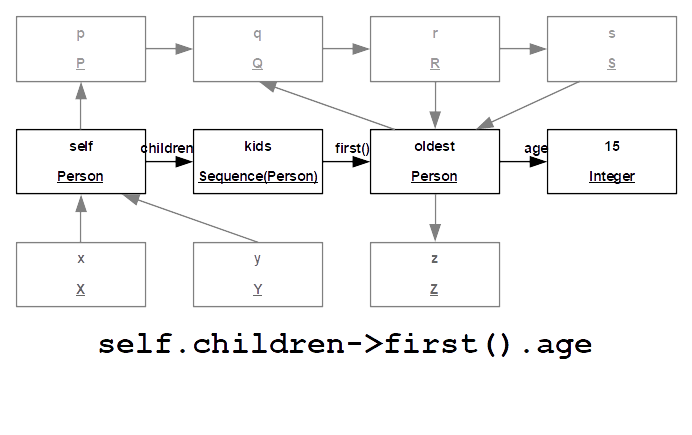
\includegraphics[width=4.5in]{OCLNavigation.png}
	\end{center}
	\vspace{-40pt}
	\caption{OCL Navigation}
	\label{fig:OCLNavigation}
\end{figure}

Figure~\ref{fig:OCLNavigation} shows a system comprising some arbitrary instances \verb$p$, \verb$q$, ... with correspondingly arbitrary types \verb$P$, \verb$Q$, .... In the center row, four objects of interest to an example expression are given more meaningful names and types to show how the example expression steps from node to node in a regular way even though the expression involves collection, operation and datatype complexities.

To keep OCL simple, we want to exploit this fundamental simplicity by providing a metamodel that suits OCL rather than contorting to accommodate the eccentricities of UML. The problem of OCL::Constraint or UML::Constraint is solved. There is always an OCL::Constraint, and an OCL::Class and an OCL::Feature that is the basis for an OCL::Property and OCL::Operation and OCL::Iteration ... OCL has its own metamodel that is designed to suit OCL free from the limitations of UML or EMOF or Ecore or XSD.

In order for OCL to co-exist with another technology such as UML, it is obviously necessary to perform a transformation of the user's UML metamodel into the equivalent OCL metamodel, for which the term Pivot was coined by the Dresden OCL \cite{Dresden-OCL} team and endorsed by the Pivot-based Eclipse OCL prototype.

The need for this transformation may seem like a burden, but it proves to be a major simplification. Without such a transformation, support for OCL for N different technologies requires N variants of the OCL tooling each adjusted to the eccentricities of that technology. In contrast a single variant of the Pivot OCL tooling is possible supported by N transformations each of which normalizes the eccentricities of its technology to the Pivot OCL formulation. UML stereotypes no longer pollute the whole of OCL, rather a Stereotype is converted to a regular OCL classifier with regular OCL features.

%The figure is clearly a graph in which the nodes can be modeled as instances of classes or as values of specialized classes often called datatypes. These concepts are adequately supported by a variety of metamodel representations.

%Edges are more troublesome, since an edge is meaningless without two nodes to define its ends. A minimal modeling of a bidirectional edge that links two nodes identifies the pair of ends. EMOF and Ecore do exactly this with their \verb$Property$ and \verb$EReference$ classes. Unfortunately UML, on which OCL~2 is based, is much more complicated. The edge is modeled by an \verb$Association$ with the ends modeled by \verb$AssociationEnd$s in UML~1 or \verb$Property$s in UML~2. UML adds the even more powerful confusion of an \verb$AssociationClass$ to treat the edge as a node. The UML complexity is clearly excessive for a simple regular OCL treatment.

A further complexity arises with unidirectional edges for which, given a known starting instance, it is only necessary to identify the far edge. EMOF and Ecore may therefore have a property contained by the source instance and referencing the remote instance. UML also supports unidirectional edges, but changes the containment of the unnavigable end to the association.

As a specification language, it is important for OCL expressions to be able to navigate in both directions~\cite{Willink-Opposites}. But this was not possible using EMOF (or Ecore) until I caused a \verb$Tag$ (or \verb$EAnnotation$) solution to be adopted.

The diverse UML, EMOF or Ecore modeling of edges are all clumsy and a poor basis for a friendly OCL representation. The irregularities are easily normalized away during a transformation to the normalized Pivot metamodel which always has a pair of \verb$Property$ instances to define a bidirectional link between \verb$Class$es and a single \verb$Property$ instance to define the unidirectional link from a \verb$Class$ to a \verb$DataType$ value.

%The state objects are easily modeled as \verb$Class$ instances with \verb$DataType$-valued \verb$Property$ slots. The link between objects can be minimally modeled by a \verb$Property$ at each end of the link. The link `end' class is adequately modeled by a \verb$Property$ in EMOF or \verb$EReference$ in Ecore. UML however models the link as well and so imposes a nearly redundant \verb$Association$ class with \verb$AssociationEnd$s in UML~1 or \verb$Property$s in UML~2 for the ends. For OCL, modeling the link is completely unnecessary; there is no need for a navigation step to stop halfway for a look around. When there really is such a need, UML has the more powerful confusion of an \verb$AssociationClass$ which adds additional unnecessary complexity to the OCL specification. Once adherence to the UML specification is abandoned, \verb$AssociationClass$es can be normalized as regular OCL classes with regular OCL properties for all their possible accesses. \verb$Association$s can be eliminated except perhaps for a lazy reification as a regular OCL \verb$Class$ for backward compatibility with some wacky OCL that really does stop halfway along a link.

%The foregoing dismissal of \verb$Association$ neglects one important complexity; the support for unnavigable opposites. In OCL~2, all links are navigable in both directions regardless of any selective naming or visibility in the user's metamodel. In UML~2, navigable ends are modeled as \verb$Property$ contained by a \verb$Class$, but the \verb$Property$ for an unnavigable end is contained by the \verb$Association$. Unnavigable ends could not be represented in EMOF (or Ecore) until I caused a \verb$Tag$ (or \verb$EAnnotation$) solution to be adopted. These diverse solutions are clumsy and easily normalized away during a transformation to the normalized Pivot metamodel.

\subsubsection{XMI}

The OCL~2 specification calls for model interchange between OCL tools using XMI but provides no clues as to how this is achieved. There appears to be a naive assumption that if there is an OCL metamodel, XMI will just work. Not so.

XMI elaborates XML's ability to serialize a tree-structure by introducing the  \verb$xmi:id$ element and corresponding references to support the graph-structures formed by cross-references in a model.

But a reference requires the \verb$xmi:id$ to exist. Unfortunately, when an OCL expression traverses an unnavigable opposite, the serialization of the \verb$PropertyCallExp$ needs to reference a property that does not exist in EMOF (or Ecore) and which exploits the unusual association-containment in UML.

The ability to extend classes with additional operations and properties poses a further challenge for XMI serialization, since the additional features are not available to be referenced as part of the original class.

More fundamentally, when a type, corresponding to for instance \verb$Set(String)$, is referenced that reference must resolve to the same definition as a similar reference from elsewhere. No overall pool of shared definitions is specified. In UML, template instantiations are performed on demand so that there may be both \verb$My::Set(String)$ and \verb$Your::Set(String)$ without any clarity as to whether they are distinct types or not.

\paragraph{Resolution}

Since OCL~2 has survived without XMI for 20 years, we could just eliminate this specification point, but given a sensibly designed metamodel, XMI should be easy. Efficient tooling for OCL-based languages such as MOFM2T or QVT will however suffer if XMI support for OCL is not possible.

The problem with serialization of the non-existent unnavigable opposite may be resolved by introducing an \verb$OppositePropertyCallExp$ class to the metamodel whose reference is to the navigable property in the other direction. Internally the normalization to the Pivot OCL metamodel can ensure that all such opposites do exist. Similar opposite modeling extensions are needed in QVT.

The Pivot-based Eclipse OCL solves the problem of locating additional features in closed classes by introducing the concept of a Complete Class that is an overlay of same-hierarchically-named closed classes. This supports open classes by overlaying as many closed classes as required. Unfortunately it has the unpleasant corollary for the tooling that accesses to Classes must redirect to their Complete Classes to ensure that any additions from sibling Classes are not overlooked.

The Pivot-based Eclipse OCL solves the problem of unique definitions by `clarifying' UML semantics to specify that the namespace hierarchy of collection, lambda, primitive, tuple types and template specializations are to be ignored. \verb$My::Set(My::String)$ and \verb$Your::Set(Your::String)$ are therefore the same type. Saving a model to XMI relocates all the shared definitions by adding an \verb|$orphanage$| package to host e.g. \verb|$orphanage$::Set(String)|. Loading from XMI relocates the contents of the many incoming \verb|$orphanage$| packages to a single global internal \verb|$orphanage$| package. Each distinct type is modeled by a distinct singleton in the Pivot representation.

\subsection{Tooling Problems}

Some aspects of the OCL language / specification cause difficulties for tooling that far exceed any convenience they may afford to users.

\subsubsection{Coherent Grammar}

Just about the first thing any toolsmith will look for when tooling a language is its grammar.

\paragraph{OCL~1.1 Grammar}

In the early days of language tooling, it was understandable that languages could have bad properties such as the notorious dangling-else ambiguity which all C/Java programmers learn about the hard way. However that all changed with the advent of LALR support tools such as yacc~\cite{YACC} which diagnose parsing problems as well as generating an efficient parser.

With the availability of yacc, it is inexcusable for any language to fail to provide a yacc grammar. The OCL~1.1 grammar dates from 1997 (22 years post-yacc). It is an EBNF grammar that can be converted to LALR form without too much trouble. Converting to LALR form reveals a multiplicity bug, a name conflict and lexer comments that are easily resolved. It also reveals a shift/reduce conflict for the expression/declaration ambiguity that we consider in Section~\ref{Expression/Declaration syntax ambiguity}.

The OCL~1.1 grammar is bad; it is incompatible with standard tooling. If LALR tooling had been used, the OCL syntax would have been adjusted.

The free parser advertised by the specification is no longer available from the IBM website. It is no longer possible to determine how the ambiguity was resolved.

\paragraph{OCL~2.1 Grammar}

At least the OCL~1.1 grammar exists as a nearly coherent whole; it can be cleaned up from a cut and paste from the specification PDF. For OCL~2.0, which is only a draft, the grammar was split up and interleaved with inherited and synthesized attribute rules. Distinct rules `clarify' each different form of navigation. This introduces many ambiguities necessitating some disambiguation rules. These difficulties are aggravated by partial name refactorings corresponding to work in progress tracking UML~1 to 2 evolution. Further difficulties arise from incomplete evolution to accommodate qualified names and static operations.

Eventually I have come to accept that the OCL~2.x grammar and CS rule specifications are not fit for purpose. Each implementer is obliged to empathize with the spirit of the specification and code accordingly. It is not surprising that few tools fully support the complexities of unnavigable opposite navigation or association classes.

I developed a yaccable version of the OCL~2 grammar for inclusion in the OCL~2.3 revision, but retracted it at the last moment when it became clear that it was biased in favor of the left recursion typical of LALR tools and against LL tools such as Xtext~\cite{Eclipse-Xtext}.

\paragraph{Resolution}

Obviously there should be a grammar that accurately specifies the language and which is demonstrably compatible with standard tools.
 
\subsubsection{Expression/Declaration syntax ambiguity}\label{Expression/Declaration syntax ambiguity}

The OCL syntax is primarily an expression language that elaborates external declarations with constraints or bodies; the declarations come from outside.

However OCL may provide a local declaration using the distinctive \verb$let...in...$ syntax or embedded with an iterator call: \verb$isUnique(n | n)$.

The \verb$let...in...$ syntax has an irritating dangling-in difficulty for an LALR grammar parsing \verb$let...let...in...in...$. This can be solved by duplicating the expression grammar to ensure that the recursion takes precedence.

The iteration syntax poses a potentially infinite look-ahead challenge to distinguish the first and second \verb$n$'s in \verb$isUnique(n | n)$. The first (declaration) \verb$n$ may be elaborated as multiple iterators with non-trivial type declarations. The second (expression) \verb$n$ may be elaborated with arithmetic operations and recursive iterations.

The look-ahead must traverse the entire declaration to detect the \verb$|$ separator to distinguish the explicit iterator \verb$isUnique(n | n)$ from the implicit iterator short-form \verb$isUnique(n)$.

\paragraph{Resolution}
 
The bad grammar should have been detected by a yacc-like tool. The ambiguous declaration syntax should have been redesigned before it was released to the world. Now we have to introduce a probably breaking change to cure it. 

The easiest solution is to use a distinctive `here-comes-a-declaration' keyword. To some extent \verb$let$ already does this.

One possibility is therefore to require the long form \verb$isUnique(n | n)$ to be rewritten as \verb$isUnique(let n in n)$ so that a \verb$let$ without an initializer defines an iterator and a \verb$let$ with an initializer is the conventional local let variable.

Another possibility is to introduce a new \verb$var$ keyword supporting a prefix declaration as in \verb$isUnique(var n; n)$. This ability to prefix a declaration to an OCL expression could render the let-expression redundant by rewriting

\begin{verbatim}
    let x = ... in let y = ... in  ...
\end{verbatim}

as

\begin{verbatim}
    var x := ...; var y := ...; ...
\end{verbatim}

The above are two suggestions for eliminating the declaration/expression ambiguity. There are no doubt others.

Any change should support the pattern matching evolution discussed at Aachen \cite{OCL-Aachen} and in Section~\ref{Patterns}.

%The former approach is incompatible with our goal of a simple re-usable grammar, so a textual syntax change is unavoidable.

%The major syntax problem arises through the introduction of prefix declarations for a long form iteration call such as

%\begin{verbatim}
%aCollection->forAll(e1, e2 | ...)
%\end{verbatim}

%This requires undue look-ahead through the iterators to find the \verb$|$ that distinguishes the iterator call syntax from the similar operation call syntax

%\begin{verbatim}
%aCollection->myForAll(e1, e2)
%\end{verbatim}

%Most of the OCL syntax is freeform which is friendly but can be challenging. Where the freeform is too hard, additional keywords such as \verb$let$ or \verb$endif$ ensure that the parser knows exactly what is happening.

%If we introduce the \verb$var$ keyword for variable declarations, we can rewrite the iteration call as

%\begin{verbatim}
%aCollection->forAll(var e1; var e2; ...)
%\end{verbatim}

%in which each \verb$var ... ;$ clause is a prefix to the subsequent OCL expression. In this case the variable type can be inferred.

%This syntax can be re-used to eliminate the let syntax by rewriting:

%This change also solves the dangling-in parsing challenge that arises when let expressions are nested carelessly. This change should also unblock my failed prototype of an OCL extension to support QVTr-like patterns that in one trivial example avoids the clumsy need for an \verb$oclIsKindOf(CastX)$ immediately followed by a matching \verb$oclAsType(CastX)$.

\subsubsection{Short-circuit operators}

In many C-based programming languages short-circuit Boolean and-or operators support a guard idiom to ensure that the evaluation of a first term converts the crash that would result from evaluating the second term to not-a-failure.

\begin{verbatim}
    (x != null) && x.doSomething()
    (x == null) || x.doSomething()
\end{verbatim}

OCL appears to be much the same:

\begin{verbatim}
    (x <> null) and x.doSomething()
    (x = null) or x.doSomething()
\end{verbatim}

but since the operators are commutative the following must return the same results 

\begin{verbatim}
    x.doSomething() and (x <> null) 
    x.doSomething() or (x = null) 
\end{verbatim}

An optimizing or a multi-processor implementation may therefore evaluate the two commutative terms in arbitrary order and so be unable to avoid the crash. so the implementation must instead catch the crash from the `wrong' term and suppress it once the guard from the `right' term is determined. The not-a-failure is not necessarily avoided.

This is not what was intended when the Amsterdam Manifesto~\cite{OCL-Amsterdam} adopted the Kleene logic to support short-circuit rather than `strict' Boolean operators. The extended Truth Table for the \verb$and$ operation was and is.

\begin{center}
	\begin{tabular}{|c||c|c||c|}
		\hline
		Use Case & Input 1 & Input 2 & Output \\
		\hline
		\hline
		2-valued & false & false & false \\
		& false & true & false \\
		&  true & false & false \\
		& true & true & true \\
		\hline
		Normal Short-Circuit & false & X & false \\
		Commutated Short-Circuit & X & false & false \\
		\hline
		Residue & true & X & X \\
		& X & true & X \\
		& X & X & X \\
		\hline
	\end{tabular}
\end{center}

The table has been redrawn here to distinguish the four 2-valued Boolean cases, the two short-circuit cases and three residual cases.

In the Amsterdam Manifesto, `X' was spelled as `undefined' and was clearly described as a virtual value meaning not-yet-computed in order to explain how the two short-circuit cases yield a useful result without needing to compute a redundant and quite possibly uncomputable term.

In OCL~2.0 and 2.2, `X' is spelled as `$\bot$' to represent a \verb$null$ or \verb$invalid$ value. Whether the output is \verb$null$ or \verb$invalid$ was unclear.

In OCL~2.3, `X' is spelled as `$\epsilon$' or `$\bot$' respectively for a \verb$null$ or \verb$invalid$ Input value and explicitly just \verb$invalid$ as an Output.

In OCL~2.4, `X' is again spelled as `$\epsilon$' or `$\bot$' for an Input value but as an idempotent `$\epsilon$' or `$\bot$' as an Output.

The 2-valued cases are uncontroversial.

The Short-Circuit cases solve the problem of choosing a Truth Table row when one of the input values cannot be computed since the short-circuit rows are available for use by not-yet-computed inputs. There is no need to attempt to compute what cannot be computed.

%The Commutated Short-Circuit row is the inevitable consequence of a commutative \verb$and$ operator. While this may be mathematically elegant, it makes for a stupid implementation, since an implementation that optimizes or uses multiple processors may easily compute the `wrong' argument first. This mandates that the implementation `catch' the consequence of malfunction of the `wrong' argument and ignore it once the `right' argument yields a \verb$false$ guard. In so far as OCL evaluation is side effect free, the only observable side effect is a waste of CPU time, but any user of a debugging or tracing tool will be confused by the chaos that may arise during the redundant failing evaluation of the `wrong' argument. While there is nothing mathematically wrong with the Commutated Short-Circuit, there is nothing practically useful and many things are practically damaging. It may also surprise users, used to traditional short circuit operators, if a crash while evaluating the first term is `rescued' by a \verb$false$ second term.

In so far as the Residual Use Cases describe the propagation of the virtual not-yet-computed value there is nothing wrong with them. However program execution does not normally reify the not-yet-computed result; rather we twiddle our thumbs waiting for the computation to complete or fail.

The virtual not-yet-computed meaning of `undefined' in the Amsterdam Manifesto evolved to the actual values of \verb$invalid$ and \verb$null$ in OCL~2 so that the Residual Use Cases no longer describe not-computations but failure propagation. %For OCL~2.0 and 2.2, as clarified in OCL~2.3, the residual use cases all result in \verb$invalid$ giving the desirable alternatives of a 2-valued or crash evaluation. The only problem would appear to be that whereas in Java, an \verb$Exception$ will propagate through the calling logic by default, for OCL-based evaluation the calling logic must be `strict' to ensure the same \verb$invalid$ propagation and so avoid the need to handle more than the \verb$true$ or \verb$false$ alternatives.

%For OCL~2.4, I was persuaded by the team formalizing OCL using Isabelle that the OCL~2.3 clarification of 4-valued input, 3-valued output Boolean logic was not idempotent. The changed 4-valued output for OCL~2.4, may be more elegant mathematically but it is certainly no better practically. How can anyone justify that

%\begin{verbatim}
%    null and null
%\end{verbatim}

%is anything other than a bad Boolean evaluation? It must be \verb$invalid$, a full failure, not \verb$null$, some kind of lesser failure. I very much regret making this change and apologize. I should have made clear that OCL~2.3 Boolean operations are really 3-valued input, 3-valued output with a `strict' preprocessor that, just like Integer or String operations, treats each \verb$null$ input as \verb$invalid$.

%While the above considerations identify some strange characteristics of the OCL Boolean operators, there is nothing actually wrong, so why are users unhappy. In Java a non-trivial Boolean calculation has three outcomes \{\verb$true$, \verb$false$, \verb$crash$\} and in OCL we also have three outcomes \{\verb$true$, \verb$false$, \verb$invalid$\}. The problem must therefore be a misunderstanding. In Java the \verb$crash$ propagates and so the Java programmer can ignore it and program as if there were only the two outcomes \{\verb$true$, \verb$false$\}. The same Java programmer handling the return from an OCL-in-Java may find that e.g. the \verb$evaluateConstraint$ API returns a distinct value for each outcome, requiring the programmer to program strictness explicitly by converting the OCL \verb$invalid$ or \verb$null$ value to a Java \verb$Exception$. If the programmer does not understand about strictness, unhappiness may result. Alternatively there may be an alternative e.g. \verb$checkConstraint$ API that provides a two-valued Java result after performing the strictness check as part of its operation; the Java programmer may now be happy.

%In conclusion, much of the unhappiness may be due to poor OCL-in-Java APIs provided by OCL tools, and misunderstanding of the need for strictness by Java programmers.

Similarly the commutative and short-circuit characteristics of the Boolean operators, when implemented, conflict with the not-a-failure intent of the Amsterdam Manifesto. This causes surprise to the user of a debugging or tracing tool who may observe the chaos of a failing redundant computation, and a further surprise to a user who finds that a crashing first term is rescued by a second term. 

\paragraph{Resolution} 

This potential of the commutated short-circuit for surprise, inefficiency and implementation difficulty may justify a change to a traditional non-commutative short-circuit. It is not clear that the mathematical elegance of commutative and-or operations provide any practical benefits; they certainly provide considerable implementation difficulties. Specify that evaluation of the first term must guard the second.

%I remain puzzled that the desirable mathematical properties of commutativity and idempotency have conflicted with practicality for OCL.





%Thus \verb$false and undefined$ can be evaluated as \verb$false$ without actually computing the second argument. As a virtual value, `undefined' would be better phrased as `not yet computed'.

%The virtual value appears to solve the problems; guarding works and even appears to be `strict' in so far as all computed \verb$null$ or \verb$invalid$ values can propagate as \verb$invalid$.

%Unfortunately the Kleene logic also specifies that \verb$and$ is commutative and so \verb$undefined and false$ must also evaluate to \verb$false$. Typical implementations will evaluate the first term as \verb$invalid$ before discovering that the second term is \verb$false$. The implementation must therefore violate strictness by caching the \verb$invalid$ while the second term is evaluated allowing the \verb$undefined and false$ Truth Table entry to be used to determine the value of \verb$invalid and false$.

%The same problem can arise with the forward guard, since commutativity allows an implementation to optimize execution to evaluate arguments in either order or even concurrently.

%The need to reify the `not yet computed' virtual value and the inappropriate correlation of the actual \verb$invalid$ and \verb$null$ values with the virtual value explains many confusions in the OCL specification. 

%\subsubsection{Short-Circuit Boolean evaluation}

%Clearly commutativity is incompatible with the guard idiom and the implementation of \verb$undefined$ as a virtual value that is never reified.

%If we reject commutativity and instead use the short circuit semantics that programmers have found very satisfactory in C and its successors, the problems vanish; any actual use of \verb$null$ or \verb$invalid$ in a Boolean operation is evaluated as \verb$invalid$. The short circuit functionality allows the first argument to inhibit the unwanted computation of a \verb$null$ or \verb$invalid$ second argument.

%The functionality is `strict', however the \verb$and$, \verb$implies$, \verb$or$ operations just like \verb$if then else endif$ have sequenced and selective argument evaluation.

%\subsubsection{Guard Syntax}

%Either the guard idiom or commutativity must go, so if commutativity is paramount, a %distinct syntax must be introduced 

%\begin{verbatim}
%    (x <> null) guards x.doSomething()
%\end{verbatim}

%This would be an OCL novelty almost deliberately conflicting with a widespread practice. A new clearer explicit syntax seems a poor trade off for user confusion.

%and to determine the answer we must lookup the left and right hand value in a Truth Table. For the case where x is \verb$null$ we look up {false and invalid} to compute false. Since and is commutative there is no difference in writing

%\begin{verbatim}
%x.doSomething() and (x <> null)
%\end{verbatim}

%and entering the Truth Table at {invalid, false} to compute false.

%This is consistent with commutativity but very surprising since most languages offer asymmetric short circuit boolean operations. It is also inconvenient for practical tooling since both arguments are of equal importance and so should be evaluated prior to Truth Table lookup.

%The design decision to break strictness to support a Kleene Boolean algebra seems to offer no benefits to the user or a practical implementation. Rather it has irritated nearly everyone.

%Eclipse OCL has finally added alternative and2, implies2, not2, or2, xor2 operations that exhibit conventional strict, short-circuit 2-valued behavior. Execution and code generation is considerably enhanced.

%\subsection{2-valued Booleans and null}

%UML defines a [?] multiplicity for values that may be null in support of the very common idiom that a slot is set by a constructor to a null value and subsequently assigned a non-null value once an appropriate initialization has completed. OCL, like Java, supports this via a null value.

%A problem arises when null values appear as inputs of Boolean operations.

%With a strict interpretation, null is bad so the result is simple; null values crash. But with commutative Kleene functionality null and null gives a null result. At best this can be confusing. There are six possible logics for {true, false, null} depending on which of the alternatives is more `important' than another. I attempted to use OCL's Boolean for a 3-valued  state, but my required logic priority differed from OCL's. It would appear that since OCL's Boolean operations for null can only be suitable for one user in six,the facility should be retracted to avoid deceiving the five out of six.

%\subsubsection{Rationalization}

%How did this mess arise?

%\verb$null$ is a genuine state of a \verb$[?]$ multiplicity variable that has not been initialized with a more explicit value or which has been explicitly assigned a \verb$null$ value. The concept was inverted by Tony Hoare, endorsed by UML~1 as the value of a \verb$[0]$ multiplicity. It was reified by UML~2 using the \verb$LiteralNull$ class and as a value by OCL~2 as the \verb$null$ literal. OCL~1 did not have a \verb$null$.

%\verb$invalid$ is a genuine value that is returned when an operation such as \verb$Sequence::at()$ has malfunctioned. It was introduced as a value by OCL~2.

%`undefined' is a virtual value used to populate the Truth Table for Boolean operations where the relevant value does not need to be defined. The sleight of hand was introduced by the Amsterdam Minifesto.

%The Formal Annex for OCL defines the special value $\bot$ as the undefined value which is part of the domain of each type, and then elaborates its usage to represent the undefined (null) value or the erroneous (invalid) return. This set the disastrous precedent for treating `undefined' as the genuine \verb$null$ or \verb$invalid$ values rather than a virtual value.

%OCL~2.0 introduced the \verb$oclIsUndefined()$ operation to test whether a value is \verb$null$ and the \verb$oclIsInvalid()$ operation to test whether a value is \verb$invalid$. \verb$oclIsInvalid()$ is not a problem, it provides a mechanism to `catch' the invalid. \verb$oclIsUndefined()$ compounds the disaster. Quite apart from being redundant, \verb$= null$ is shorter and more conventional, it re-inforces the incorrect association of the word `undefined' and the value \verb$null$. Successive maintainers of the OCL specification, including myself, have sought to use only the genuine values \verb$null$ and \verb$invalid$ and rewritten text and the Truth Tables accordingly.

%As a consequence, evaluation of \verb$null and true$ uses the \verb$undefined and true$ entry and returns \verb$null$. If however `undefined' is only a virtual value, there is no Truth Table entry to support \verb$null and true$. This is a pre-condition failure and the result is therefore \verb$invalid$ giving us the strict semantics that we require.

%\subsubsection{Other Problems}

%There are too many other problems to address here. Some are listed in the `OCL~2.5' RFP~\cite{OCL-2.0-RFP} and others as part of the revisions in Section~\ref{Specification Revisions}.

\section{Evolution}\label{Evolution}

This section summarizes successful and planned work that goes beyond the narrow limitations of the specification before drawing on experience of what has failed or is at least unduly complex to make some radical suggestions as to how an OCL~3 might be specified more usefully.

\subsection{Prototyped Evolution}

We  first identify functionality that has been successfully prototyped by Eclipse OCL.

\subsubsection{Map library type}

The Map type is familiar to OO programmers but sadly missing from OCL.

\paragraph{Resolution} Implemented \cite{Willink-Map}. Provision of Map literals and joint key/value iterators is useful.

\subsubsection{Safe navigation}\label{Safe navigation}

The side effect-free characteristics of OCL make an OCL program much easier to analyze than many other languages. However many constraints suffer from problems with null navigation.

\paragraph{Resolution} The prototype exploits the \verb$[1]$ and \verb$[?]$ multiplicities of UML to distinguish not-null from maybe-null and so identify statically which expressions have a null-hazard. A \verb$?.$ safe navigation operator is introduced. The first implementation of this was almost useless for collections and so some elaborations that include specifying distinct collection and element multiplicities as in \verb$Set(String)[*|1]$ were required \cite{Willink-Safe}.

\subsubsection{Type construction / shadow types}

Users find it inconvenient that an OCL expression cannot create an instance of a type. The OCL specification also finds this inconvenient and introduces \verb$make$ operations. At first sight this is an insoluble problem because creation of a new instance creates a side effect in the memory system and OCL is side effect free.

\paragraph{Resolution} The prototype introduces the concept of shadow objects \cite{Willink-Shadow} in which the `created' object is a shared immutable re-use from a notionally infinite pre-existing pool of all possible instances. There is no side effect even though a practical implementation no doubt populates the infinite pool lazily. Once extended to a model transformation environment supporting mutations, assignment of a container to a shadow object must clone to preserve the immutability.

\subsubsection{Templates, Lambdas and Reflection}

The OCL specification uses many facilities without properly specifying them.

The collections are specified using a magic \verb$T$ that has more akin to a textual macro than a type argument. Clearly the \verb$T$ in \verb$Set(T)$ is a template parameter. If it isn't, then how does it relate to the missing support for UML template parameters?

The body of an OCL iteration call is an expression to be evaluated for each iteration. This is clearly an anonymous function definition well known to the computer science community as a lambda expression. The contorted specification of the \verb$closure$ iteration using the language of textual macro substitution is clear evidence that lambda expressions are in use.

Reflection is little used in OCL, perhaps because the OCL~2 specification has repeatedly changed the semantics of \verb$oclType()$ seemingly in an effort to find a valid way of providing access to the name of a type without imposing the baggage of a fully reflective type system.

The reflective OCL~1 seems much clearer and supports the usage within some of the OCL~2 flatten() constraints.

\begin{verbatim}
post: result =
   if self.oclType().elementType.oclIsKindOf(CollectionType)
   then ...
\end{verbatim}

\paragraph{Resolution} An implementation that fully supports templates, lambdas and reflection avoids the need for clumsy workarounds to provide the half-baked functionality that fails to satisfy user expectations. Once lambda expressions exist, lambda types and so lambda variables follow, allowing function bodies to be passed arbitrarily rather than just as the special case of an iterator body.

\subsection{Pending Evolution}

Some problems have been tackled but not completed.

\subsubsection{Fail-safe execution}\label{Fail-Safe OCL}

Safe navigation, as described in \ref{Safe navigation}, prevents the most common OCL execution failures but not all. Divide-by-zero is very rare in OCL, but index-out-of-bounds with ordered collections is far from rare, particularly for users who accidentally use the 0-based indexing of implementation languages rather than the 1-based specification policy. With these problems detected, an OCL expression can be guaranteed not to require the complexities of \verb$null$ or \verb$invalid$; a Boolean expression is provably two-valued.  

\paragraph{Resolution} This is work in progress to support code generation for QVTr where run-time handling failures is very undesirable; a failure during a transformation is a failure and obscure when it happens. A compile-time check that proves that a failure is impossible is more useful for the user and allows for simpler and faster generated code.

A little integer value flow analysis is needed to prove that e.g. \verb$x->at(x->size()-1)$ is safe only if \verb$x$ is provably not empty.

A form of assertion will be needed for expressions that are too complicated for practical symbolic analysis.

\subsubsection{Precision}

As a specification language, OCL specifies unbounded precision for its ideal Integer and Real calculations. This is clearly unrealistic and inefficient for many practical applications where 16 bits is often enough for counters and sequence indexes.

In practice, the type declarations of the model slots from which values are read provides a strong clue as to what precision is appropriate, but it is only a clue. To avoid implementation guesswork, there should be a mechanism for OCL evaluations to specify precision, overflow and underflow behavior.

\paragraph{Resolution}

Executable UML \cite{UML-Executable} provided a plausible mechanism to model precision, but it was not adopted by UML~2. It did however influence the OCLforUML profile \cite{Willink-OCLforUML} that users apply to their UML models.

The precision aspects of the profile are mostly a documentation convenience. The profile was developed primarily to identify null-free Collections in support of the safe navigation work. See Section~\ref{Safe navigation}.

\subsubsection{Patterns}\label{Patterns}

At the Aachen \cite{OCL-Aachen} workshop, an OCL enhancement to support pattern matching was discussed. At its most trivial, this would allow the verbose idiomatic test-and-cast usage

\begin{verbatim}		
    if x.oclIsKindOf(CastX)
    then x.oclAsType(CastX).doSomething()
    else null
    endif
\end{verbatim}

which requires two library calls and two specifications of the \verb$CastX$ type to be simplified as a pattern-match-guarded action:

\begin{verbatim}
    if var castX : CastX := x
    then castX.doSomething()
    else null
    endif
\end{verbatim}

The success, or failure of the match of the value of \verb$x$ expression against the \verb$castX : CastX$ pattern determines the direction taken by the \verb$if$. Within the \verb$then$ branch, the successfully bound \verb$castX$ variable can be used with its matched \verb$CastX$ type.

\paragraph{Resolution}

Some work has been done on this, but it foundered on the Expression/Declaration syntax ambiguity discussed in Section~\ref{Expression/Declaration syntax ambiguity}. Elaborating the declaration syntax was too hard. Introduction of the \verb$var$ keyword could unblock this impediment.

The work also identified that the QVTr template syntax was probably suitable for re-use as a pattern syntax and that conversely introducing a different syntax for OCL would be very damaging to the QVTr grammar as a whole.

\subsubsection{Libraries}

One of the most impressive characteristics of Java is how its Object polymorphism enabled it to launch with powerful Collection libraries that have grown and grown. C++ lagged horribly. OCL still lacks support for standard or user libraries, the most obvious of which would be a maths library.

\paragraph{Resolution}

The OCL and QVTr Standard Libraries are implemented by models for the Pivot-based Eclipse OCL and QVTd, however an attempt to provide a tutorial demonstrating a maths library proved much harder than expected. Allowing a user to write \verb$atan2(x, y)$ challenges the support for static operations whereas \verb$Maths::atan2(x, y)$ is familiar to Java users but hardly worthy of a specification language.

\section{An OCL~3 tooling Proposal}\label{OCL~3 tooling Proposal}

If OCL is to be easy to extend, it must have a clear specification with a clear architecture. Once these are clear there are opportunities for an implementation to exploit this clarity to produce a correspondingly clear tooling implementation. The clear implementation facilitates selective `borrowing' by a user who really wants to rewrite, and selective overriding by a user who is interested in re-use.

Unfortunately the significant omissions from the OCL specification result in the rather vague architecture shown in Fig~\ref{fig:OCL2Architecture} that practical implementations may ignore completely or revise in proprietary fashion. The net result is poor quality incompatible tools that discourage re-use.

\subsection{The big problems}

A solution to many of the problems has been suggested above and successfully prototyped as part of the Pivot-based Eclipse OCL. However there are two areas where the prototype solution is unpleasant; the prototype has tried too hard to maximize conformance to a perhaps over-enthusiastic interpretation of the letter of the specification.

%No matter whether extension occurs for source or compiled functionality, it is very desirable that OCL maximizes its ability to be-re-used by providing genuinely re-usable grammars, models and rules. This is the approach that has been pursued by the Pivot-based Eclipse OCL with extension for QVTc or QVTr. However the poor quality of the OCL and QVT specifications have made the extension rather hard.

%There is an opportunity to revisit the specification to facilitate some significant simplifications for tooling and to enable the original goals to be realized.
 
%The specification, or at least the interpretation of the specification, needs to be revisited to allow the prototype to be significantly simplified, to allow alternative accurate implementations to exist, and to ensure that the specification is clear to all.

\subsubsection{Open classes}

The ability to add attributes and operations to open classes is difficult to support when their AS representation is to be just like similar attributes and operations defined in a model based on closed classes.

Many modeling capabilities such as Acceleo~\cite{Eclipse-Acceleo}, ATL~\cite{Eclipse-ATL} and QVTo~\cite{Eclipse-QVTo} support additional features as helper operations and helper attributes. They are clearly useful and an important aid to modularization of non-trivial OCL constraints. The deliberate avoidance of such helpers by the UML~2.5~\cite{UML-2.5} specification leads to some long unreadable repetitive OCL expressions. This clearly demonstrates their utility.

However we only need helper features and so a reversion to the OCL~1.x pseudo-features would suffice. Once the need for fully open classes goes, the inconvenience of the prototype's Complete Class overlay of closed classes in the prototype can be resolved; externally the user's metamodel may use a closed class semantics. Internally the normalized Pivot model may open the class to inject the additional features.

%With an AS serialization that serializes references as descriptors rather than resolved references, the problem of where the referenced definition exists is no longer a problem.
 
%This problem led Eclipse OCL to prototype a solution whereby a complete-Class was an overlay of same-named partial-Classes enabling the additional definitions to be overlaid on the primary definition and serialized in a similar fashion. This gives a powerful but non-trivial transitive Package merge capability for same-URI packages. Is it really necessary?



%If a user's requirement is to use OCL as-is then they just need to program their application and exploit the OCL tool support APIs. The user code will be responsible for providing models.

%More likely, the user wants a bigger language of which OCL just forms a part. Model Transformation Languages are examples of this. This lends itself to two alternate architectures.

%The OCL support could be a re-usable component with a limited amount of parameterization with the application independently coded and struggling with the limited parameterzations and APIs. This is the approach offered by the Classic Eclipse OCL and used by Eclipse QVTo and Eclipse Acceleo.

%Alternatively the larger application uses similar technology to the OCL tooling so that each OCL aspect is extended allowing the larger application to be generated as a coherent whole. This is the approach taken by the Pivot Eclipse OCL and used by Eclipse QVTd to support QVTc and QVTr.

%If OCL is to be useful building block it must easily re-usable


\subsubsection{Two metamodels}

%The need for two metamodels, a CS model resembling the grammar and an AS model for interchange and use by tooling causes considerable complexity, much aggravated by ambiguities in the grammar and general vagueness.

%The prototype has two metamodels and it is unpleasant, in some respects doubling complexity.

%The obvious solution of replacing two metamodels by one is not feasible since the requirements for efficient usage by AS consumers is not compatible with that of grammar compatibility with the CS. We can however move to one and a bit metamodels.

%Once we accept the need to make OCL much simpler and much more re-usable, what should be changed? 
The main complexity comes from the two distinct CST and ASG metamodels aggravated by the poorly designed grammar that mandates non-standard tooling to support disambiguation with untimely semantic insights. The grammar can be improved to solve the aggravations, but two metamodels seem unavoidable since the CST is similar to the grammar to ease parsing. The ASG is a compact and sensible information model to facilitate efficient use for execution and analysis.

The two metamodels are mostly isomorphic with AS classes such as \verb$IfExp$ with condition/then/else children replicated by a \verb$IfExpCS$ CS class with three equivalent children. Many of the differences arise from the need for the CS to accommodate ambiguities until there is sufficient context to select the unambiguous AS variant. Other difficulties arise from the way in which references to elements such as types are modeled.

Exactly the same problems occur in the QVT specifications and so I sponsored Adolfo Sanchez-Barbudo Herrera's EngD~\cite{Sanchez} to provide automated tooling to assist in the awkward CS2AS conversion. This work started in 2013 and so at that time we still lacked the confidence or insight to call out the OCL~2 specification approach as fundamentally unsound.

We can now challenge the presumption that two metamodels are necessary.
Once we follow the resolution of Section~\ref{Expression/Declaration syntax ambiguity} to revise the grammar and eliminate ambiguities we are left with just the element referencing issue, which we can resolve by trimming our two metamodels not quite to one metamodel, but to one and a bit. %Figure~\ref{fig:OCL3Architecture} shows a simpler and more regular architecture that might be adopted for OCL~3. We will contrast it with Figure~\ref{fig:OCL2Architecture} to indicate how problems vanish.
%The obvious solution of replacing two metamodels by one is not feasible since the requirements for efficient usage by AS consumers is not compatible with that of grammar compatibility with the CS. We can however move to one and a bit metamodels.

\subsection{Modeling a Type Reference}

The ability to make one and a bit metamodels work relies on a seemingly trivial aspect of the metamodeling.

In the concrete syntax of many languages the letter-sequence for a built-in type such as \verb$String$ may occur many many times. This does not mean that there are many copies of the built-in type, rather that there are many descriptions of the built-in type. It is the responsibility of the tooling to ensure that only one such type does exist so that each reflective usage of the type shares a single definition.

Similarly the letter-sequence for a synthesized type such as \verb$Set<String>$ may occur many times. Once again, it is the responsibility of the tooling to ensure that only one underlying type definition exists.

\begin{figure}
	\begin{center}
		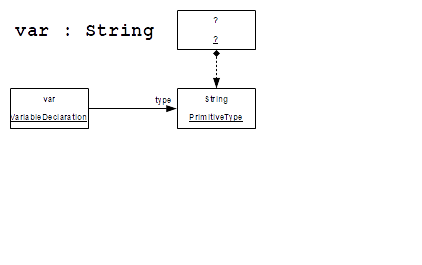
\includegraphics[width=4.5in]{OCL2TypeReference.png}
	\end{center}
	\vspace{-110pt}
	\caption{OCL~2 Type Reference}
	\label{fig:OCL2TypeReference}
\end{figure}

When UML models a type, it uses \verb$TypedElement$ as the abstraction of all model elements that have types, \verb$Type$ as the abstraction of all types and the \verb$TypedElement::type$ property as the mechanism by which the \verb$TypedElement$ references its \verb$Type$. Fig~\ref{fig:OCL2TypeReference} shows how the OCL metamodel uses this property to associate \verb$String$ as the primitive type of a \verb$VariableDeclaration$. Since the \verb$String$ primitive type may be used by many definitions, it cannot be contained by the \verb$VariableDeclaration$ rather it must be contained elsewhere. For a built-in type we can ignore the problem as a bit of implementation magic.

However once we model use of a \verb$Set<String>$ this approach does not work since not all possible template specializations can be built-in, rather a shared instance of \verb$Set<String>$ must be modeled. The UML metamodel provides two solutions to this problem. For types, the user is required to create an explicit specialization somewhere so that it can be referenced as many times as necessary. This approach is fine for an informal specification but fails when my subsystem has one definition of \verb$Set<String>$ and your subsystem has another. For non-types, where creation of an instance elsewhere is too inconvenient, UML has another idiom. There may be two alternative references such as the non-containment \verb$TemplateParameterSubstitution::actual$ and the sibling containment \verb$TemplateParameterSubstitution::ownedActual$ giving the modeler the freedom to use whichever is convenient and the user the inconvenience of a derived property to select the appropriate property.

The UML approach is `right' in so far as it attempts to force the singleton existence of type definitions, but `wrong' in that the enforcement is incomplete and inappropriate for a specification language. A unique definition is only a necessity for an implementation. A specification language may refer many times to the unique type.

In contrast if we examine the modeling for the same problem in Ecore, we find that \verb$ETypedElement::eType$ is very similar to UML's \verb$TypedElement::type$. However when Ecore evolved to support Java generics, an \verb$EGenericType$ rag-bag was added. Each \verb$EGenericType$ is a descriptor for a required type contained by the new \verb$ETypedElement::eGenericType$ property. Ecore, although practically an implementation language, evolved to support type descriptions. The OCL metamodel, emulating UML, is cursed with UML's inappropriate modeling of type singletons. 

Recognizing the different ways in which a type reference can be modeled, we can see that the `CS' metamodel must model the multiple descriptions of a type whereas the `AS' must model the single definition of that type. We do not however need two metamodels if our one and a bit metamodels provides a pair of properties; a primary type description property for use by consumers of the `CS' metamodel such as parsers, and a secondary derived type definition property for the `AS' consumers such as code generators and validators.

We are left with a design decision to make in regard to interchange using XMI. If the interchange exposes the `AS' content, we can interchange fully resolved definitions but have difficulties ensuring that the two parties to the interchange are able to share globally unique definitions. If instead the interchange is limited to the `CS' content only, type descriptions are shared and each party is free to use its own policies to resolve the descriptions to its own locally unique definitions. % Omission of the 'AS' content is exactly what happens when the additional content uses derived properties.

Since the `CS' content is exchanged with other tools we will refer to this as the `external' perspective of our one and a bit metamodels, and to the private `AS' content as `internal'

\begin{figure}
	\begin{center}
		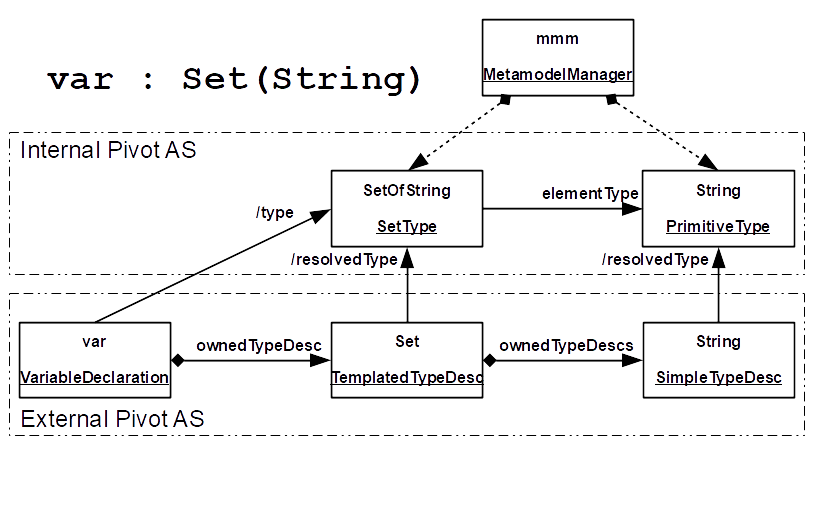
\includegraphics[width=4.5in]{OCL3TypeDescriptor.png}
	\end{center}
	\vspace{-40pt}
	\caption{Possible OCL~3 Type Descriptor}
	\label{fig:OCL3TypeDescriptor}
\end{figure}

Fig~\ref{fig:OCL3TypeDescriptor} shows the `external' and `internal' modeling for our \verb$Set<String>$ example. On the bottom row we show the external type description in which the \verb$VariableDeclaration$ owns a description comprising a \verb$TemplatedTypeDesc$ named \verb$Set$ which in turn owns a \verb$SimpleTypeDesc$ named \verb$String$. On the middle row we show the internal type definitions comprising the singleton \verb$PrimitiveType$ named \verb$String$ that is referenced by the singleton \verb$SetType$ named \verb$SetOfString$. The  derived \verb$resolvedType$ properties of the many external perspective descriptions reference the singletons of the internal perspective.

The package and model ownership of the singletons is omitted in the interests of clarity. Transitively a single \verb$MetamodelManager$ is the container of all singleton definitions.

\subsection{Overall OCL~3 Architecture}

Having solved the problem of two metamodels, we can now see how the various components of the Overall architecture shown in Fig~\ref{fig:OCL3Architecture} collaborate to provide a satisfactory solution to many of the problems in Fig~\ref{fig:OCL2Architecture}. 

\begin{figure}
	\begin{center}
		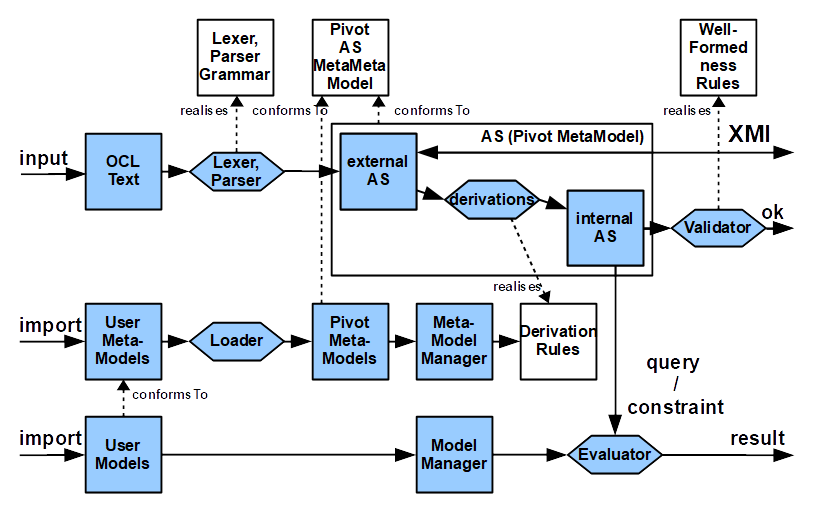
\includegraphics[width=4.5in]{OCL3Architecture.png}
	\end{center}
	\caption{Possible simplified OCL~3 Architecture}
	\label{fig:OCL3Architecture}
\end{figure}

\paragraph{MetamodelManager}

At the heart of the architecture is the MetamodelManager that is responsible for the normalized singleton Pivot representations within
the Pivot Metamodels.

When an `import' is required, the MetamodelManager locates the referenced user metamodel, and activates the appropriate Loader to convert it to the normalized Pivot form ensuring that any shared declarations use the appropriate singleton definitions. As part of the loading process, any esoteric user elements such as UML's Stereotype or AssocationClass are normalized to the simple classifier-feature internal representation.

When a `lookup' is required by a Derivation Rule to resolve an element description to its unique element definition, the lookup is performed by querying the Metamodel Manager.

OCL~2 neglects to specify how metamodels are imported, but it does specify an \verb$Environment$ class to perform queries at a particular scope. Unfortunately a new \verb$Environment$ instance is created and then modified for each nested scope created by for instance a let-expression. This is clearly not OCL. The \verb$Environment$ instances are passed down the CST so that each node has its own instance with all possible definitions. This is very inefficient and involves many mutations and so side effects.

Between imports, the Metamodel Manager is logically immutable lazily exposing only what is required from a nationally infinite pool of all possible definitions. A lookup is therefore much more easily resolved by an immutable search up the AS for what is required rather than a churning push down of everything that could be required.

In addition to the imported user metamodels, the Metamodel Manager supervises the loading of the standard Pivot metamodel, if the user requires reflective functionality, and the OCL Standard Library. Each of these loads may be overridden to support use of a customized Pivot or Library.

\paragraph{Specification}

The transparent boxes show the functionality to be provided by grammars and models in the specification. In contrast to Fig~\ref{fig:OCL2Architecture} we see that the Disambiguation Rules have vanished since the grammar ambiguities are removed. This allows standard parser tooling to be used. The lookup Rules have also vanished, or rather migrated to the Derivation Rules that perform a simple query to convert the element description parsed from the source text to the element definition required by the internal AS.

There is just one (and a bit) metamodels.

The Well-formedness rules are substantially unchanged.

\paragraph{Basic Parsing}

The second row of Fig~\ref{fig:OCL3Architecture} shows the OCL text input model being parsed by standard lexer and parser tooling configured by the specified grammar. The resulting External perspective of the Pivot AS is suitable for interchange using XMI.

This basic parsing can potentially be performed without the aid of a MetmodelManager. This may be convenient for some novel OCL re-use cases, but in practice the services of the advanced tooling will be essential for any form of validation or completion assist in an editor.

\paragraph{Advanced Tooling}

Advanced tooling activates the MetamodelManager to covert all the references in the external AS to the unique definitions of the internal AS. This enables tools that exploit the OCL such as Validators or Evaluators to provide enhanced capabilities.

\paragraph{Model Manager}

Analogously to the use of the MetamodelManager to supervise all metamodels, the ModelManager supervises the models for use by the evaluator. In addition to the obvious task of loading required models, it also supports all the possible forms of feature access that may be used in those models. For the simplest form of property access this may just require that a value be obtained from a slot and converted to the appropriate Boolean/Integer/Real/String representation. In more complex cases the reified form of an applied stereotype may need to be navigated to obtain a slot value from the instance of the stereotype.

%Returning to the proposed architecture in Figure~\ref{fig:OCL3Architecture}, we see the metamodel management on the third row with a defined import mechanism for the user metamodels followed by a loader transformation that converts the user's preferred metamodel representation to the normalized Pivot representation. The loading and storage is supervised by the \verb$MetamodelManager$ which also provides the requisite abilities to query the metamodels to locate a required metamodel element from its description.

%The \verb$Loader$ transformation accommodates alternative user metamodel representations and normalization of their eccentricities

%OCL~2 neglects to specify how metamodels are imported, but it does specify an \verb$Environment$ class to perform queries at a particular scope. Unfortunately a new \verb$Environment$ instance is created and then modified for each nested scope created by for instance a let-expression. This is clearly not OCL. The \verb$Environment$ instances are passed down the CST so that each node has its own instance with all possible definitions.

%Once loading has completed the \verb$MetamodelManager$ instance and its children are logically immutable; the infinite pool of all possible synthesized types already exists. It is just necessary to return a reference to the required one. Obviously a practical implementation will create them lazily on demand.

%The very inefficient and non-OCL push-down of \verb$Environment$ instances can be replaced by an immutable search up of the AS.

%On the top row we have similar transparent boxes for the specification specified behavior, but with the CS and AS unified in the single Pivot AS metamodel. The CS2AS rules have evolved to the derivation rules managed by the MetamodelManager.

%The second row shows the similar lexing and parsing functionality but only requires the external perspective of the metamodel which is interchanged through XMI.

%The third row shows the metamodel management with imported metamodels on the left passing through a loader that normalizes the user representation to the Pivot representation supervised by the MetamodelManager.

%On the bottom row user models are loaded and supervised by a ModelManager that orchestrates the denormalized access to the user models on behalf of the normalized evaluation.

%The Evaluator and Validator are examples of detailed OCL tooling that use the internal perspective of the Pivot AS metamodel that is lazily populated from the external perspective using the Derivation Rules.




%The most glaringly missing, greyed out, part of the OCL~2 architecture is the support for user and built-in metamodels (and models). The missing import mechanism, root \verb$Environment$ and treatment of specialized constructs such as \verb$Stereotype$ must be resolved.

%The problem with XMI for OCL~2 is the need to serialize references to awkward definitions. With the two perspective AS suggested above, the external perspective comprises descriptors for the definitions avoiding the difficulties. After an XMI load, the descriptors can be resolved in a very similar fashion to the lazy resolution after parsing.

%Another source of UML complexity arises from \verb$Stereotype$s. These are completely ignored by the OCL specification. The UML~2 specification provides only a minute example from which to extrapolate the, perhaps only possible, coherent design. \verb$Stereotype$s are readily normalized to \verb$Class$es and \verb$Property$s to facilitate regular OCL navigation.

%In summary, the core of the OCL Pivot metamodel needs just well-defined \verb$Class$ and \verb$Property$ classes.


%\subsubsection{Unified Metamodel}

%The second row of Figure~\ref{fig:OCL3Architecture} is similar to Figure~\ref{fig:OCL2Architecture} in so far as OCL Text is lexed and parsed and eventually validated. However the need for a non-standard parser is eliminated by revising the grammar to avoid the need for disambiguation rules. The distinct CST and ASG are replaced by the external and internal perspectives of a unified Pivot metamodel. The descriptive properties of the external perspective, like the CST, are populated by the parser. The definitive properties of the internal perspective are somewhat like the ASG, however since they share the same host classes, no transformation is needed. Rather a derivation rule is lazily invoked to derive the internal transient property by resolving the description from the external perspective to its definition for the internal perspective.


%CST and ASG are replaced by the external and internal perspectives of a unified Pivot metamodel. 



%The transformation between CST and ASG is replaced by derivation rules that elaborate the descriptive external perspective with the definitive internal perspective. The parser populates the external perspective properties with descriptions that are lazily resolved by a derivation rule to their internal perspective definition when each derived transient property is accessed.

%The utility of the element descriptions may be demonstrated by considering the way in which a type reference is handled by the OCL~2 and OCL~3 architectures.

%\begin{verbatim}
%    var : String
%\end{verbatim}

%The partial AS for OCL~2 is shown in the Figure~\ref{fig:OCL2TypeReference} Instance Diagram. The \verb$VariableDeclaration$ named \verb$var$ has a \verb$type$ reference to the \verb$PrimitiveType$ named \verb$String$. The containment of the \verb$PrimitiveType$ is unclear but no doubt magically available from somewhere. The reference-to-type is simple and obvious but a containment problem appears once we consider a declaration with a synthesized type; one that must be constructed rather than just magically available.

%\begin{verbatim}
%    var : Set(String)
%\end{verbatim}

%The \verb$VariableDeclaration::type$ must now point to some type that is constructed or re-used on behalf of the reference. The OCL~2 specification provides no clues, although in response to the issue that I raised, \verb$ExpressionInOCL::generatedType$ was added in OCL~2.2 without any indication of how it solves the problem or ensures uniqueness.

%The \verb$MetamodelManager$ brings order to this anarchy by supervising the model elements that may be built-in to the tooling, form part of a library, form part of a user metamodel or which may be constructed on demand to satisfy the need for a unique definition of a synthesized type. Figure~\ref{fig:OCL3TypeDescriptor} shows a \verb$MetamodelManager$ with transitive containment via omitted packages and models to the built-in library \verb$PrimitiveType$ instance and the synthesized \verb$SetType$ instance.

%In order to isolate the parser from the complexities of locating unique definitions, the \verb$VariableDeclaration::type$ property is changed to a derived property that is part of the internal perspective. The \verb$VariableDeclaration::ownedTypeDesc$ external perspective property is populated by the parser with a description of the referenced type. This description is locally contained by the referencing \verb$VariableDeclaration$ and so may be as complicated as necessary. In the example, the \verb$Set$ is parsed as a \verb$TemplatedTypeDesc$ parameterized by a \verb$Set$ name and \verb$String$ template parameter. The template parameter is parsed as a \verb$SimpleTypeDesc$ parameterized by a \verb$String$ name. Each type descriptor has a lazily resolved \verb$TypeDesc::resolvedType$ derived property as its internal perspective. 




%In this case an adjustment to the AS to accommodate direct parsing solves a significant XMI serialization issue for free. No change to the textual concrete syntax is necessary.

%An example of the benefits of revisiting the AS can be seen by considering the problem of referencing a type as in:

%It seems obvious that the AS should have a \verb$VariableDeclaration::type$ property so that the instance of \verb$Variable$ has a \verb$type$ reference to the type whose name is \verb$String$. 

%This is shown in Figure~\ref{fig:OCL2TypeReference} and is exactly what the OCL~2 specification defines. The Figure is a UML instance diagram with additional decorations to show compositions. The containment of the PrimitiveType is unclear.

%The design is poor since its support for synthesized template types is troubled.

%\begin{verbatim}
%var : Set(String)
%\end{verbatim}

%Somehow the a definition of \verb$Set(String)$ must be located to terminate the \verb$VariableDeclaration::type$ reference. Where is that definition? Presumably it must be unique, so there is an additional problem in ensuring uniqueness if \verb$Set(String)$ is referenced from multiple XMI serializations. The OCL specification provides no answers, although in response to the issue that I raised, \verb$ExpressionInOCL::generatedType$ was added in OCL~2.2 without any indication of how it solves the problem or ensures uniqueness.

%The problem is that in the textual concrete syntax we have type descriptions such as \verb$Set(String)$ that are repeated for every distinct usage. \verb$String$ too is a six letter type description that converts to a primitive type.

%To facilitate parsing we need a model that supports type descriptions; the non-normative CS classes do exactly this for OCL~2. But to facilitate OCL execution we would like a more streamlined AS representation that references the described type. Currently the conflict is resolved by incurring an awkward CS2AS conversion phase.

%If we accept that a little bloat of the OCL AS is acceptable, we can have a \verb$VariableDeclaration::ownedTypeDesc$ composed property and a \verb$VariableDeclaration::type$ derived transient property. The composed \verb$VariableDeclaration::ownedTypeDesc$ property owns an object tree that describes the referenced type and is constructed directly by the parser similar to the OCL~2 CS. The derived \verb$VariableDeclaration::type$ property references the resolved type just as the 




%many supervises the Pivot metamodel representation normalized by the loader transformation from the user's preferred metamodel representation. 





%Fig~\ref{fig:OCL3Architecture} shows a simpler and more regular architecture that might be adopted for OCL~3. 

%\subsubsection{Summary}

%The \verb$MetamodelManager$ supervises the Pivot metamodel representation normalized by the loader transformation from the user's preferred metamodel representation. 

%The distinct CST and ASG are replaced by a single dual-perspective Pivot AS.

%The external aspects comprise element descriptors populated by the parser. The external aspects can be interchanged using XMI. 

%The internal aspects comprise the uniquely resolved elements for each descriptor. The resolutions use derived transient properties whose body invokes a \verb$MetamodelManager$ query using the reserved variable \verb$mmm$.

%The transient internal uniquely resolved aspects are determined by derived properties that use the \verb$MetamodelManager$ to resolve element descriptions to the normalized elements loaded from user metamodels. 

%The \verb$ModelManager$ performs model loading and value normalization on behalf of the evaluator.

%Revision of the grammar and AS to avoid ambiguities avoids the need for non-standard parser disambiguation.

%Replacing the distinct CST and ASG by external and internal aspects of a single Pivot AS avoids the need for non-standard parser resolution and facilitates interchange with XMI.
%But how? Important classes such as \verb$Package$, \verb$Class$, \verb$Property$, \verb$Operation$, \verb$Constraint$ are missing. The specification just loosely suggests that the equivalents from your favorite metamodeling language can be used, specifically assuring that the EssentialOCL is compatible with EMOF even though EMOF (and Ecore) has no \verb$Constraint$ class at all. Some Ecore tools struggle to extend Ecore with a missing \verb$EConstraint$. Eclipse OCL struggles with magic overloads of \verb$EAnnotation$.







\section{Conclusion}\label{Conclusion}

We have shown how the well-intentioned upgrade of the simple but useful OCL~1 specification went astray as part of the UML~2 activities. We have identified that draft work-in-progress was accidentally adopted as the OMG OCL~2 specification.

We have drawn on personal experiences to explain why OCL tool implementers treated the OCL~2 specification with unwarranted reverence and struggled to implement it as faithfully as possible.

It is a pity that it has taken so long to recognize the OCL~2 specification for the disaster that it is.

We make proposals for an OCL~3 that can almost be seen as going back to OCL~1 and then moving forwards again to avoid the mistakes of OCL~2.

This appears to leave the OCL community with a three-way choice:
\begin{itemize}
\item Do nothing. USE and Eclipse OCL and so OCL will fade away.
\item Evolve existing OCL tool(s). Current teams are inadequate.
\item Develop a new OCL. There is no team.
\end{itemize}

Any future progress surely depends on a credible specification. This requires significant work, which may be mitigated if some simplifications are made.

Eclipse OCL could evolve to prototype the simplifications, but only if that is what the community wants.
\backmatter

\bibliographystyle{alphaurl}
\bibliography{OCLReflections}

\abouttheauthors

\begin{acknowledgments}
Many thanks to Horacio Hoyos Rodriguez and the anonymous reviewers for helpful comments on an inadequate initial submission.
\end{acknowledgments}

\end{document}


